\documentclass{article}
\usepackage[margin=1in]{geometry}
\usepackage{microtype}
\usepackage{setspace}
\usepackage{amsmath}
\usepackage{parskip}
\usepackage{amssymb}
\usepackage{graphicx}

\graphicspath{{../public/}}

\parskip=4ex
\date{}
\author{}

\title{12.7 Triple Integrals in Spherical Coordinates}

\begin{document}
  \maketitle
  \textbf{Introduction}\\
  Another useful coordinate system in three dimensions is the spherical coordinate system, simplifying evaluating triple integrals over regions bounded by spheres or cones.

  \textbf{Spherical Coordinates}\\
  The spherical coordinates $ (\rho,\theta,\phi) $ of a point $ P $ is shown below. $ \rho = | OP |$ is the distance from the origin to $ P $, $ \theta $ is the same angle as in cylindrical coordinates, and $ \phi $ is the angle between the positive $ z $ axis and the line segment $ OP $.

  \begin{center}
    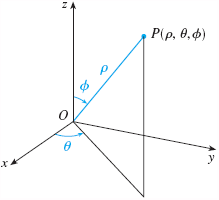
\includegraphics[width=5cm]{12_7_1}
  \end{center}

  Note that
  \[
    \rho \ge 0 \qquad 0 \le \phi \pi
  \]

  To convert from spherical to rectangular coordinates
  \[
    x = \rho \sin{\phi}\cos{\theta} \qquad y=\rho\sin{\phi} \sin{\theta} \qquad z=\rho\cos{\phi}
  \]

  The distance formula shows that
  \[
    \rho ^{2} = x^{2}+y^{2}+z^{2}
  \]

  This equation is used to convert from rectangular to spherical coordinates

  \textbf{Ex 1}\\
  Convert $ (2,\frac{\pi}{4},\frac{\pi}{3}) $ from its spherical coordinate form to rectangular coordinates
 \[
   \begin{gathered}
   x=\rho \sin{\phi}\cos{\theta}= 2\sin{\frac{\pi}{3}}\cos{\frac{\pi}{4}}= \sqrt{\frac{3}{2}}\\
   y=\rho\sin{\phi}\sin{\theta} = 2\sin{\frac{\pi}{3}}\sin{\frac{\pi}{4}}=\sqrt{\frac{3}{2}}\\
   z=\rho\cos{\phi}=2\cos{\frac{\pi}{3}}=1\\
   \boxed{(2,\frac{\pi}{4},\frac{\pi}{3}) \to (\sqrt{\frac{3}{2}},\sqrt{\frac{3}{2}},1)} 
   \end{gathered}
 \]

 \textbf{Ex 2}\\
 Convert the rectangular coordinate point $ (0,2\sqrt{3}, -2) $ into its spherical coordinate form
 \[
   \begin{gathered}
   \rho = \sqrt{x^{2}+y^{2}+z^{2}} = \sqrt{0+12+4}=4\\
   \cos{\phi}= \frac{z}{\rho}=-\frac{1}{2} \qquad \phi = \frac{2\pi}{3}\\
   \cos{\theta}=\frac{x}{\rho\sin{\phi}}=0 \qquad \theta=\frac{\pi}{2}\\
   \boxed{(0,2\sqrt{3},-2 ) \to (4,\frac{\pi}{2},\frac{2\pi}{3})}
   \end{gathered}
 \]
 
 \textbf{Evaluating Triple Integrals with Spherical Coordinates}\\
 In spherical coordinate systems, the counterpart of a rectangular box is a spherical wedge
 \[
   E=\{ (\phi, \theta, \phi) | a \le \rho \le b, \alpha \le \theta \le \beta, c \le \phi \le d \}
 \]

 where $ a \ge 0, \beta-\alpha \le 2\pi, ~\&~ d-c \le 2\pi $. 

 Though we typically divide solids into small boxes, using smaller spherical wedges yield the same result. We divide $ E $ into these smaller partitions $ E_{ijk} $ by means of spheres $ \rho=\rho_i $, half-planes $ \theta=\theta_j $, and half-cones $ \phi=\phi_k $. 

 $ E_{ijk} $ is approximately a rectangular box with dimensions $ \Delta \rho_i, \rho_i \Delta \phi_k , ~\&~ \rho_i\sin{\phi_k\Delta \theta_j}$, shown in the figure below.
  \begin{center}
    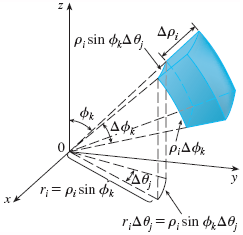
\includegraphics[width=5cm]{12_7_2} \qquad
    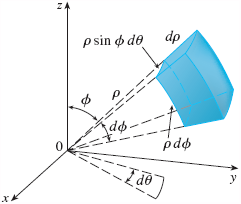
\includegraphics[width=5.5cm]{12_7_3}
  \end{center}
  
  \[
    \INT*{^{},_E,^{}}f(x,y,z)~dV\\
    \to\\
    \int^{d}_{c} \int^{\alpha}_{\beta} \int^{b}_{a} f(\rho\sin{\phi}\cos{\theta},\rho\sin{\phi}\sin{\theta},\rho\cos{\phi})\rho^{2}\sin{\phi}~d\rho d\theta d\phi 
  \]

  where $ E $ is a spherical wedge given by
  \[
    E=\{ (\phi,\theta,\phi) a \le \rho \le b, \alpha \le \theta \beta, c \le \phi \le d\}
  \]

  Which can be extended to include more general spherical regions such as
  \[
  E=\{ (\rho, \theta, \phi) | \alpha \le \theta \le \beta, c \le \phi \le d, g_1(\theta,\phi) \le \rho \le g_2(\theta,\phi)\}
  \]

  Usually spherical coordinates are used in triple integrals when surfaces such as cones and spheres form the boundary of the region of integration.
 
  \textbf{Ex 3}\\
  Evaluate $ \INT*{^{},_B,^{}} e^{(x^{2}+y^{2}+z^{2})^{\frac{3}{2}}}$, where $ B $ is the unit ball
  \[
    B=\{ (x,y,z) | x^{2}+y^{2}+z^{2} \}
  \]
  \[
    \begin{gathered}
      \INT*{^{},_B,^{}}e^{(x^{2}+y^{2}+x^{2})^{\frac{3}{2}}}~dV = \int^{\pi}_{0} \int^{2\pi}_{0} \int^{1}_{0} e^{\rho^{3}}\rho^{2}\sin{\phi} ~ d\rho d\theta d\phi = \boxed{\frac{4\pi(e-1)}{3}}
    \end{gathered}
  \]
\end{document}
